% 建议使用 XeLaTeX 或 LuaLaTeX 编译(中文与公式支持更佳)
\documentclass[UTF8,zihao=-4]{ctexart}

\usepackage[a4paper,margin=2.5cm]{geometry}
\usepackage{amsmath, amssymb, amsthm}
\usepackage{bm}
\usepackage{hyperref}
\usepackage{graphicx}
\usepackage{caption}
\usepackage{listings}
\usepackage{xcolor}
\usepackage{float}
\usepackage{placeins}
\graphicspath{{figures/}}

\lstdefinestyle{code}{
  basicstyle=\ttfamily\small,
  numbers=left,
  numberstyle=\tiny,
  numbersep=8pt,
  keywordstyle=\color{blue},
  commentstyle=\color{teal!70!black},
  stringstyle=\color{orange!70!black},
  showstringspaces=false,
  breaklines=true,
  frame=single,
  framerule=0.3pt,
  rulecolor=\color{black!15}
}
\lstset{style=code}

\title{局部离群因子(LOF):原理、公式、应用与实战}
\author{}
\date{\today}

\begin{document}
\maketitle

\section{引言}
局部离群因子(Local Outlier Factor, LOF)通过比较样本与其邻域的局部密度来检测异常点。如果某个点的密度显著低于邻居,则其 LOF 得分偏高,被视为潜在离群。与全局距离阈值不同,LOF 能在密度不均的数据中识别异常。

\section{原理与公式}
\subsection{$k$ 距离与可达距离}
给定样本 \(\mathbf{x}\) 及邻域大小 \(k\),定义 \(k\) 距离 \(d_k(\mathbf{x})\) 为 \(\mathbf{x}\) 到第 \(k\) 个最近邻的距离。样本 \(\mathbf{x}\) 对邻居 \(\mathbf{y}\) 的可达距离为:
\begin{equation}
\operatorname{reach}_k(\mathbf{x}, \mathbf{y}) = \max\{ d_k(\mathbf{y}), \lVert \mathbf{x} - \mathbf{y} \rVert_2 \}.
\end{equation}

\subsection{局部可达密度与 LOF}
\(\mathbf{x}\) 的局部可达密度(LRD)定义为与邻域 \(N_k(\mathbf{x})\) 之间可达距离的平均值的倒数:
\begin{equation}
\operatorname{lrd}_k(\mathbf{x}) = \left( \frac{1}{|N_k(\mathbf{x})|} \sum_{\mathbf{y} \in N_k(\mathbf{x})} \operatorname{reach}_k(\mathbf{x}, \mathbf{y}) \right)^{-1}.
\end{equation}
LOF 得分则比较邻居密度与 \(\mathbf{x}\) 的密度:
\begin{equation}
\operatorname{LOF}_k(\mathbf{x}) = \frac{1}{|N_k(\mathbf{x})|} \sum_{\mathbf{y} \in N_k(\mathbf{x})} \frac{\operatorname{lrd}_k(\mathbf{y})}{\operatorname{lrd}_k(\mathbf{x})}.
\end{equation}
若 LOF 接近 1,说明密度与邻居类似;明显大于 1 则可能是异常点。

\subsection{超参数与实践注意事项}
参数 \(k\) 控制检测的局部范围:过小易受噪声干扰,过大则模糊局部结构。距离度量、特征缩放及类别变量处理都会影响效果。由于 LOF 得分是相对指标,需要结合业务容忍度或预估的污染率选取阈值。

\section{应用与技巧}
\begin{itemize}
  \item \textbf{网络入侵检测}:在高维日志中发现异常流量模式。
  \item \textbf{工业监控}:定位传感器漂移或故障导致的低密度点。
  \item \textbf{欺诈分析}:识别显著偏离同类群体的客户行为。
  \item \textbf{实用建议}:先标准化特征,尝试多组 \(k\) 参数,分析 LOF 得分分布,并结合领域知识确认异常告警。
\end{itemize}

\section{Python 实战}
脚本 \texttt{gen\_lof\_figures.py} 构造包含簇结构与零散异常的数据,使用 scikit-learn 的 \texttt{LocalOutlierFactor} 进行训练,并输出得分热图与直方图以展示离群分布。
\begin{lstlisting}[language=Python,caption={脚本 gen_lof_figures.py 片段}]
from sklearn.neighbors import LocalOutlierFactor

lof = LocalOutlierFactor(n_neighbors=35, contamination=0.08)
pred = lof.fit_predict(points)
scores = -lof.negative_outlier_factor_
\end{lstlisting}

\section{实验结果}
\begin{figure}[H]
  \centering
  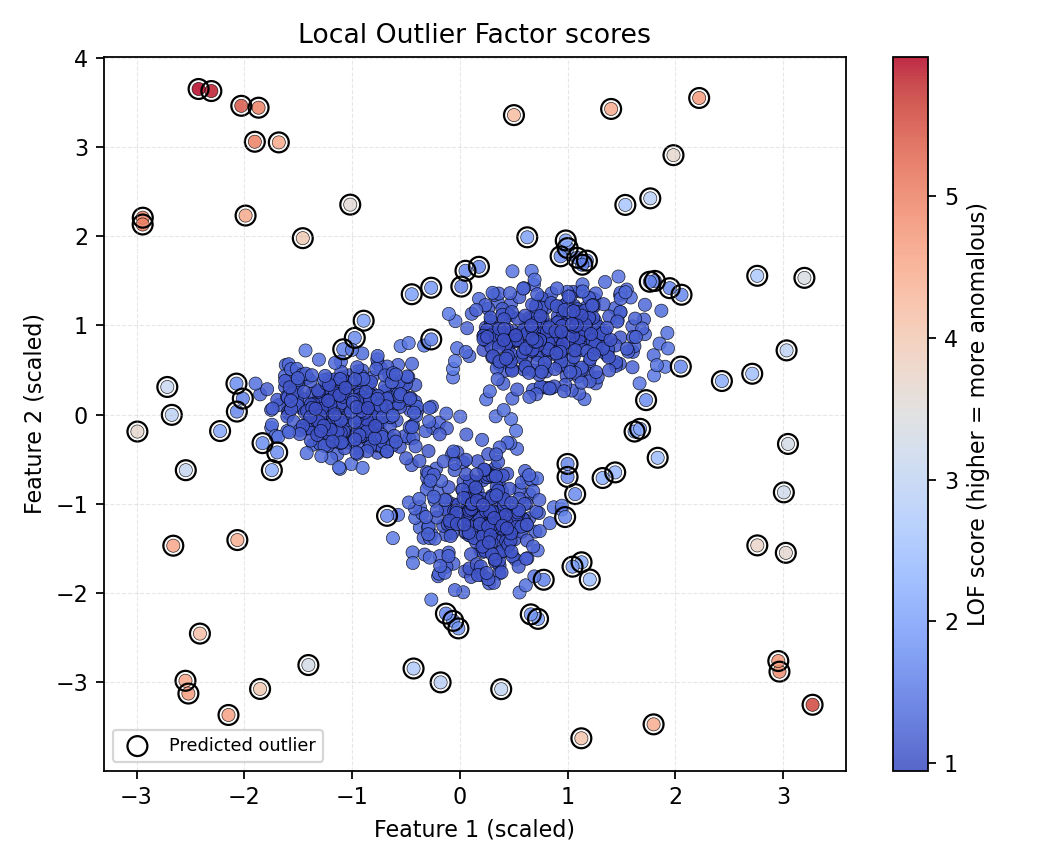
\includegraphics[width=0.82\linewidth]{lof_decision_map.png}
  \caption{LOF 得分热度图,得分越高表示局部密度越低}
  \label{fig:lof_decision_map_cn}
\end{figure}

\begin{figure}[H]
  \centering
  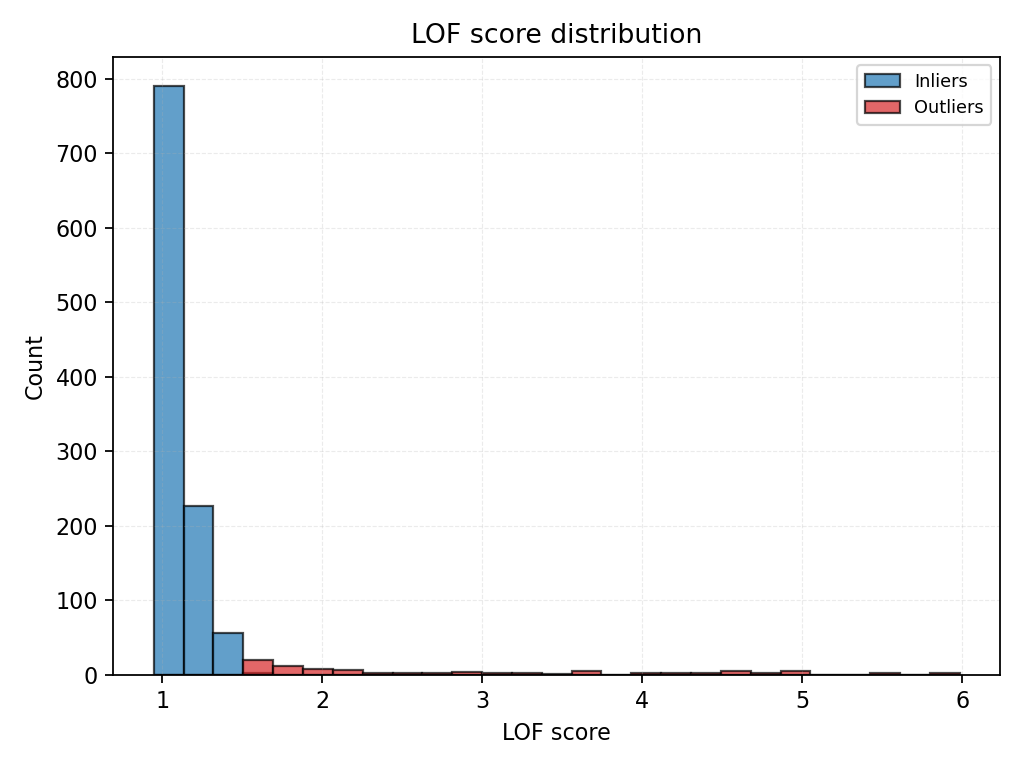
\includegraphics[width=0.78\linewidth]{lof_score_hist.png}
  \caption{LOF 得分直方图,对比模型识别的正常与异常样本}
  \label{fig:lof_score_hist_cn}
\end{figure}

\FloatBarrier
\section{总结}
LOF 通过局部密度比值识别离群点,特别适合密度分布不均的数据。合理的特征缩放、邻域参数选择及可视化分析,有助于在安全、工业与金融场景中构建稳定的异常检测系统。示例展示了 LOF 如何将零散样本与密集簇区分开来,并根据得分分布选择阈值。

\end{document}